
\documentclass[12pt,a4paper]{article}
\usepackage[T2A]{fontenc}
\usepackage[utf8]{inputenc}
\usepackage[english]{babel}
\usepackage[left=2cm,right=2cm,top=2cm,bottom=2cm]{geometry}
\usepackage{cyrtimes}
\usepackage{graphicx}
\usepackage{listings}
\usepackage{indentfirst}
\usepackage{tabularx}
\usepackage{hyperref}
\usepackage{setspace}
\begin{document}
\lstset{
numbers=left,
tabsize=4,
breaklines=true,
title=\lstname,
}
\title{Status report for IMT4002}
\author{(Nataliia Uvarova, Oleksandr Yakushev, 13HMACSA)}
\date{2014}
\maketitle
\onehalfspacing

%----------------------------
\section{Overview}
After considering two service architectures, SOAP and REST, we decided to go with the latter.
Our RESTful service is implemented in Python by using \href{http://flask.pocoo.org/}{Flask} microframework.
It greatly simplifies handling HTTP requests and lets focus on the client side more.

Client-side is written mostly in Javascript together with \href{http://www.angularjs.org/}{AngularJS} framework.
AngularJS has many advantages over using plain JS, as it strongly promotes MVC pattern,
supports declarative programming for the UI and allows to avoid many of the Javascript ugly parts.

Requirement to be able to work while offline is met by using Web Storage.
This technology was picked because of its availability in all modern browsers.

For the second part of the task we use the \href{http://leafletjs.com/}{leaflet} library
which provides nice API for maps (in particular, OpenStreetMaps).

The unimplemented yet part is ability to upload images from the client. As images should be
uploaded with other content of the note i.e.\  json data we plan to use formdata from
the XMLHttpRequest 2 standard, which allows to post any formdata. Downside of this approach (in contrast to use
non pure solution), that minimal version of the IE, that supports XHR2 is 10.

\section{RESTful service}
As the main client for the service is the web application, then REST api has
several advantages over the SOAP-bases solution.

\begin{itemize}
    \item REST is use full features of HTTP (different methods and results codes),
        thus information about client-server communication is spread between the
        method, which is asked, the result code server returns and the message itself.
        It could be good or bad depending on the application, but it is well-fitted
        to the model web-client and particulary javascript uses.
    \item the JSON is native for javascript, whereas XML could be hardly created and parsed.
    \item all modern frameworks and libraries support commnunication and retrieval data from RESTful
        service, whereas only few could work with SOAP based solution.
    \item developing RESTful service could be done much faster
\end{itemize}

There could be some reasons to use SOAP-based solution. One of the dominant -
if you should integrate with the existing infrastructure, that is already built
using SOAP. Also several programming languages has good support for SOAP, but
Python is not from that group of languages.

So as a result - Python with Flask-Restful and AngularJS, which commnunicate via JSON,
form good stack of technologies, which are compatible with each other.
It is also possible to form other stack of technologies, which is based on SOAP
(and possibly Java).

The service will allow user to create and get `notes' (rich geotagged messages). Note is basically a
dictionary (or in other words json object) which holds geocoordinates and user-provided content (text or image).

Currently our service supports the following requests:
\begin{description}
    \item[geonotes(GET)] return a list of all stored notes
    \item[geonotes(POST)] create new note. As newly created note is not fully equal to posted data.
        The provided image is represented as url for dropbox file, when information about note
        is provided for user. Because of this, the result of the POST is not only id, as
        some architectures suggest, but full note content, as it is represented in geonotes list in GET response.
    \item[geonotes/<note\_id>(GET)] return a specific note
\end{description}

Other possible operations on notes (such as edits and deletions) are not mentioned in the task, but can be implemented later via adding extra service requests.

One remark should be made about bulk operations.
Canonical REST architecture specification does not clearly define how to design bulk requests (i.e.\ bulk creates and updates).
Since the client-side will send multiple changes after the offline session, we will consider to extend service API with an ability to accept bulk requests
for faster start-up and more optimal bandwidth usage.

\section{Client-side}

Here is summarized table (based on \url{http://caniuse.com}) of the minimal
versions of popular browsers, which support features, used in client-side.

\begin{table}[h!]
    \caption{Browsers compatibility (in braces - current version)}
    \begin{tabularx}{\linewidth}{|c|X|X|X|X|X|X|X|}
        \hline
        Feature & IE (11.0) & Firefox (27) & Chrome (33) & Safari (7.0) & Opera (19) & IOS Safari (7.0) & Android Browser (4.4) \\ \hline
        XMLHttpRequest 2 & 10.0 & 26.0 & 31 & 7.0 & 19.0 & 5.0 & 3.0 \\ \hline
        Offline cache    & 10.0 & 26.0 & 31 & 7.0 & 19.0 & 3.2 & 2.1 \\ \hline
        Geolocation      &  9.0 & 26.0 & 31 & 7.0 & 19.0 & 3.2 & 2.1 \\ \hline
        \hline
        Resulting        & 10.0 & 26.0 & 31 & 7.0 & 19.0 & 5.0 & 3.0 \\ \hline
    \end{tabularx}
\end{table}

\subsection{AngularJs}

One of the neat features of AngularJs is good support for form validation and in overall
handling different form states (clean - dirty, valid - invalid). This allows to 
easily give user feedback, whether he can submit the form or not and what is the problem.

On the figures there are screenshots of offline version, which contains only form,
and on the other, this form embedded in modal dialog, which appears on click on map.

    \begin{figure}[h]
      \begin{center}
        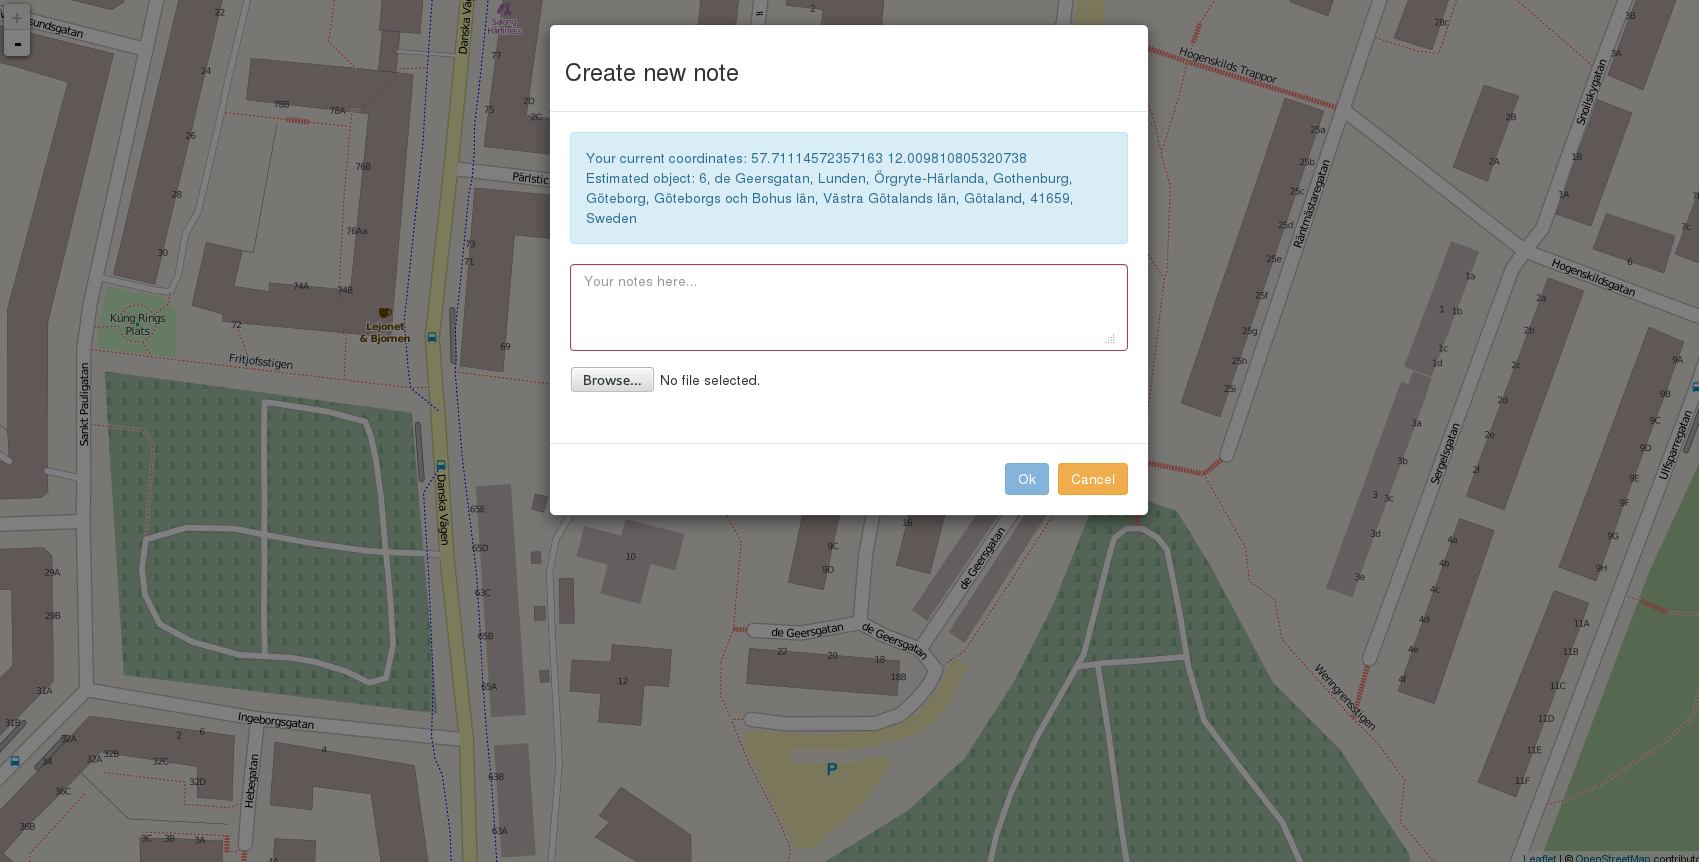
\includegraphics[width=\textwidth]{res/online}
      \end{center}
      \caption{Online version}
    \end{figure}

    \begin{figure}[h]
      \begin{center}
        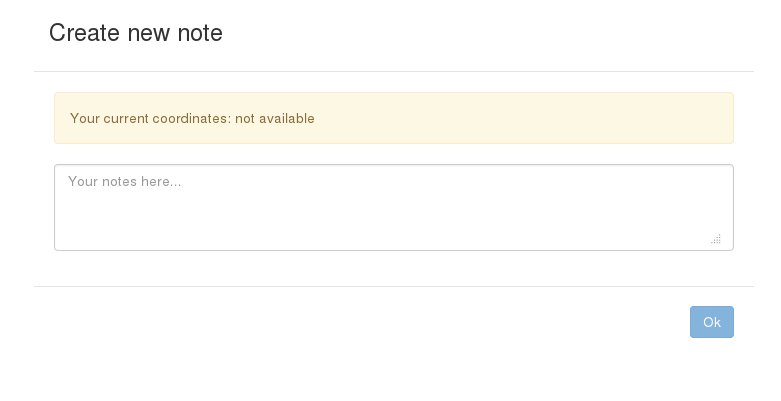
\includegraphics[width=\textwidth]{res/offline}
      \end{center}
      \caption{Offline version}
    \end{figure}

//TODO: compare with other frameworks

\subsection{Leaflet}
Leaflet is library for maps. It is mainly used for OpenStreetMaps and derivatives,
but can be used also with GoogleMaps.
Leaflet is designed with simplicity, performance and usability in mind.
It works efficiently across all major desktop and mobile platforms out of the box,
taking advantage of HTML5 and CSS3 on modern browsers while still being accessible on older ones.

Leaflet is fairly new project, compared to OpenLayers. Thus, Leaflet is much simpler to use,
the codebase is smaller, but on other hand, there is no a lot of examples, tutorials and
the community is not mature. For example, the Leaflet extension for AngularJS is quite
unmature, thus requires sometime either to extend it yourself or to use workarounds
or to fallback to plain Leaflet, which all harms the simplicity and clarity of the code.

The principal advantages of the Leaflet over OpenLayers for this project is
it is more suitable for mobile web. The codesize of the Leaflet is smaller
and there is builtin support for touch-screen events (touches are mapped to
the clicks and you can zoom map with two fingers without adding extra code).

\subsection{Cache manifest}
For providing offline version HTML5 cache manifest file is used. It is still working
draft, but has support if most recent browsers (even in mobile, except Opera Mini).

Through special manifest file, application can specify which files are required for
offline version and should be cached. Useful feature is the \textbf{FALLBACK} section,
where you can specify the replacements for particular files, when there is no network
access.

Offline version of the application has two key files different from online.
It is \textit{app.js}, which is specification of Angular application, where root
controller is specified. For online version, root controller and template renders maps
and for offline version, it is just form, where user can write his notes.

Next is \textit{services.js}, which corresponds to the model. In offline version
in should save notes to the localstorage, in the online version - send requests
to the server.

\section{DropboxAPI}
For integration with DropboxAPI, server-side synchronization is used. The reasons
for such decision are next:

\begin{itemize}
    \item it is compatible with RESTful design principle, when server can hide N-tiers architecture.
    \item simplify the client, client should not bother with setting the connection both the
server and the Dropbox
    \item simplify authorization. Since only server connects to Dropbox, the OAuth process can
be performed once and the access\_token can be stored on server.
\end{itemize}

Dropbox provides well-designed API for access with OAuth authorization.
There are three types of API, the application can use:

\begin{description}
    \item[CoreAPI] - provides access to regular file system. Allow to upload and download files.

    \item[SyncAPI] - the special API for native mobile apps, so it can sync files
        and be notified of changes.

    \item[DatastoreAPI] - provides access to special storage, designed to storage
        raw data, instead of just files. Each datastore is table of records. Each record
        is set of key-value pairs, where values can be string, numbers etc.
\end{description}

Each application that wants to have access to any API, should request an app key and
use this key in process of app authorization. Application can request two types of permissions:
first - have access to only app folder and Datastore, and second - to have access to
all files of the user.
For this application minimal permissions are enough.

Application use two DropboxAPIs: CoreAPI and DatastoreAPI.
CoreAPI is used to upload user media content (like images)
For syncing other data (like coordinates and text) DatastoreAPI is used.

// TODO: compare to other storage-service API (i.e GoogleDrive or Box)

\section{Geo names}
//TODO: about geo names

\section{Source code}
    You can find the latest version of the code on Github.
    \url{https://github.com/AAzza/geonaut}.

    \begin{description}
        \item[server/] here lives the restful server.
        \item[test\_server.py] here lives tests for server.
        \item[templates/manifest.appcache.jinja] Template for HTML5 cache manifest file.
        \item[static/index.html] entry point for the client-side.
        \item[static/js/app.js] entry point for the Angular applicaion.
        \item[static/js/app\_offline.js] entry point for the offline Angular applicaion.
        \item[static/js/controllers.js] file with all controllers, which contains all application logic.
        \item[static/js/services.js] storage and model for online version (perform request to server).
        \item[static/js/services\_offline.js] storage and model (store data to localstorage).
        \item[static/js/partial/] directory with html templates
    \end{description}
\end{document}
